\documentclass[a4paper,11p]{memoir}

%\pdfoutput=1

\newlength{\figwidth}
% FINAL
%\setlength{\figwidth}{88mm}
% DRAFT
\setlength{\figwidth}{0.65\textwidth}


\usepackage{color}
\definecolor{links}{rgb}{0.7,0,0}   % red
\definecolor{urls}{rgb}{0,0,0.8}    % blue
\definecolor{cites}{rgb}{0,0,0.8}   % blue

\usepackage[colorlinks,hyperindex,linkcolor=links,citecolor=cites,urlcolor=urls]{hyperref} % generates colored links in pdf file
%---------------------------------------------------------
% styles and other macros
\usepackage[nosort]{cite}        
\usepackage{url} 
\usepackage[intlimits]{amsmath}
%\usepackage{bbm}
\usepackage{graphicx}
\usepackage{paralist}
\usepackage{verbatim}
\usepackage{amsfonts}
\usepackage[stretch=16,shrink=16,step=4]{microtype}
\usepackage{amssymb}
%\usepackage{vmr-symbols-rndbold}
%\usepackage{standard-macros}
%\safemath{\txant}{m_{\mathrm{t}}} %number of transmit antennas
\safemath{\txantalt}{\widetilde{m}_{\mathrm{t}}}
\safemath{\rxant}{m_{\mathrm{r}}} %number of receive antennas
\safemath{\cohtime}{n_{\mathrm{c}}} %time-frequency coherence length (in symbol times)
\safemath{\bl}{n} %blocklength
\safemath{\err}{\epsilon} %error rate
\let\snr\undefined
\safemath{\snr}{\rho} %snr
\safemath{\tfdiv}{l}  %amount of time-frequency diversity available (number of independent fading realizations observed over a codeword)
\safemath{\ncod}{M}
% \let\complexset\undefined
% \safemath{\complexset}{\amsbb{C}}
% \safemath{\realset}{\amsbb{R}}
% \safemath{\naturalset}{\amsbb{N}}
% \safemath{\Rmax}{R^*}
% \safemath{\Rmaxala}{R^*\sub{ala}}
% \safemath{\Rmaxp}{\Rmax(\tfdiv,\cohtime,\epsilon,\snr)}
% \safemath{\Rmaxalap}{\Rmaxala(\tfdiv,\cohtime,\epsilon,\snr)}
% \safemath{\Cerg}{C\sub{erg}}
% \safemath{\Cout}{C\sub{out}}
% \safemath{\Pout}{P\sub{out}}
% \safemath{\diversity}{d}
% \safemath{\multiplexing}{r}
% \safemath{\Pustm}{P_{\rmatX}^{\mathrm{u}}}
% \safemath{\maxantalt}{p}
% \safemath{\minantalt}{q}
% \safemath{\altgamma}{\widetilde{\gamma}}
% \newcommand{\infoden}[2]{\ensuremath{\imath\lefto({#1};{#2}\right)}}   % expectation
% \safemath{\alshouffle}{e}



\def\matn{\mathcal{N}}
\def\matcn{\mathcal{CN}}
\def\matc{\mathcal{C}}
%\newcommand{\safemath}[2]{\newcommand{#1}{\ensuremath{#2}\xspace}}
\def\txant{m_{\mathrm{t}}} %number of transmit antennas
\def\txantalt{\widetilde{m}_{\mathrm{t}}}
\def\rxant{m_{\mathrm{r}}} %number of receive antennas
\def\cohtime{n_{\mathrm{c}}} %time-frequency coherence length (in symbol times)
\def\bl{n} %blocklength
\def\err{\epsilon} %error rate
\def\snr{\rho} %snr
\def\tfdiv{l}  %amount of time-frequency diversity available (number of independent fading realizations observed over a codeword)]
\def\ncod{M}
\def\tr{\mathrm{tr}}
\def\PP{\mathbb{P}}
\def\EE{\mathbb{E}}
\def\complexset{\mathbb{C}}

%*******************************************************************************
%!TEX encoding =  

\begin{document}


\title{SPECTRE\\
Short Packet Communication Toolbox\\[1cm]
Version 0.2}

\author{Contributors (alphabetic order):\\
Austin Collins, Giuseppe Durisi, Victoria Kostina, \\Johan \"Ostman, Yury Polyanskiy, Ido Tal, Wei Yang\\[10pt]
e-mail: \url{fblcode-list@mit.edu}}




\maketitle

\begin{abstract}

Shannon theory describes fundamental limits of communication and
compression systems. Classic closed-form results
(such as the well known $\log(1+\mathrm{SNR})$ formula)   apply only to the regime of infinite blocklength
(infinite packet size/delay). For finite blocklengths, no closed-form results are usually
obtainable, but there  exist tight upper and lower bounds, as well as
approximations. This manual describes numerical routines for  computing
these bounds and approximations for some popular channel and
source models.

The toolbox is under development and the participation of additional
members of the information and communication theory communities in
this endeavor is warmly welcomed!
\end{abstract}
\newpage
\tableofcontents

\newpage
%%%%%%%%%%%%%%%%%%%%%%%%%
\chapter{Motivation}
%
  In his 1948 landmark paper, Claude E. Shannon demonstrated that communication with arbitrarily small probability of error is feasible if, and only if, the communication rate is below the so called channel capacity. 
  To achieve this result, codes with large packet size (blocklength) must be employed. 
 Shannon's channel capacity has served as a useful guideline to design wireless communication systems.

In some applications, however, a more refined analysis of the interplay between packet-error probability, communication rate, and packet size is required.
  This may occur in emerging applications, such as massive machine-to-machine communication for metering, traffic safety, and telecontrol of industrial plants, together with real-time data transfer to enable remote wireless control (tactile internet), which may require the exchange of short packets, sometimes under stringent latency and reliability constraints.
  
Finite-blocklength information theory, a subfield of information theory that benefitted from seminal contributions from Shannon, Strassen, and Dobrushin, among others, is currently a very active field of research. 
Nonasymptotic achievability and converse bounds on the \emph{maximum coding rate} achievable for a given packet size and packet error probability are now available for several channel models that are relevant for wireless communication systems, such as the AWGN channel, the quasi-static Rayleigh fading channel, and the Rayleigh block-fading channel.
The purpose of this toolbox is to provide numerical routines for the computation of these bounds.
In the next chapters, we provide a bare-bone manual, which describes the routines available in this toolbox.



% subsection contributors (end)
%%%%%%%%%%%%%%%%%%%%%%%%%
\chapter{The real AWGN channel}


General info:
\begin{itemize}
\item Maintainer: Y. Polyanskiy \url{<yp@mit.edu>}

\item Main references: \cite{PPV08}

\item Example: See Fig.~\ref{fig:awgn_example} 

\item Channel model:
	$$ Y_j = X_j + Z_j, \quad j=1,\ldots,n $$
	\begin{itemize}
	\item Codewords are real: $x_j \in \mathbb{R}, j=1,\ldots,n$
	\item Noise: $Z_j \sim \matn(0,1)$ iid.\\
	\item Power constraints: Each codeword $x^n$ satisfies
			$$ \sum_{j=1}^n |x_j|^2 \le n P $$
	\end{itemize}

\item Common input/output arguments:
\begin{enumerate}
\item \verb|P| -- input argument; parameter of the power constraint (so $P=10$ is $SNR=10~dB$).
\item \verb|epsil| -- block probability of block error.
\item \verb|lm| or \verb|Lms| -- output argument; $\log_2 M$, log-size of codebook (base-2 information units). 
\item \verb|n| -- input argument; blocklength.\\
		For slow functions that do not support vectorized arguments.
\item \verb|Ns| -- input argument; vector of blocklengths.
\end{enumerate}
\end{itemize}


\begin{figure}
\centering
\begin{verbatim}
	> plot_v3(10, 0.001, 1, 100:20:1000)
\end{verbatim}
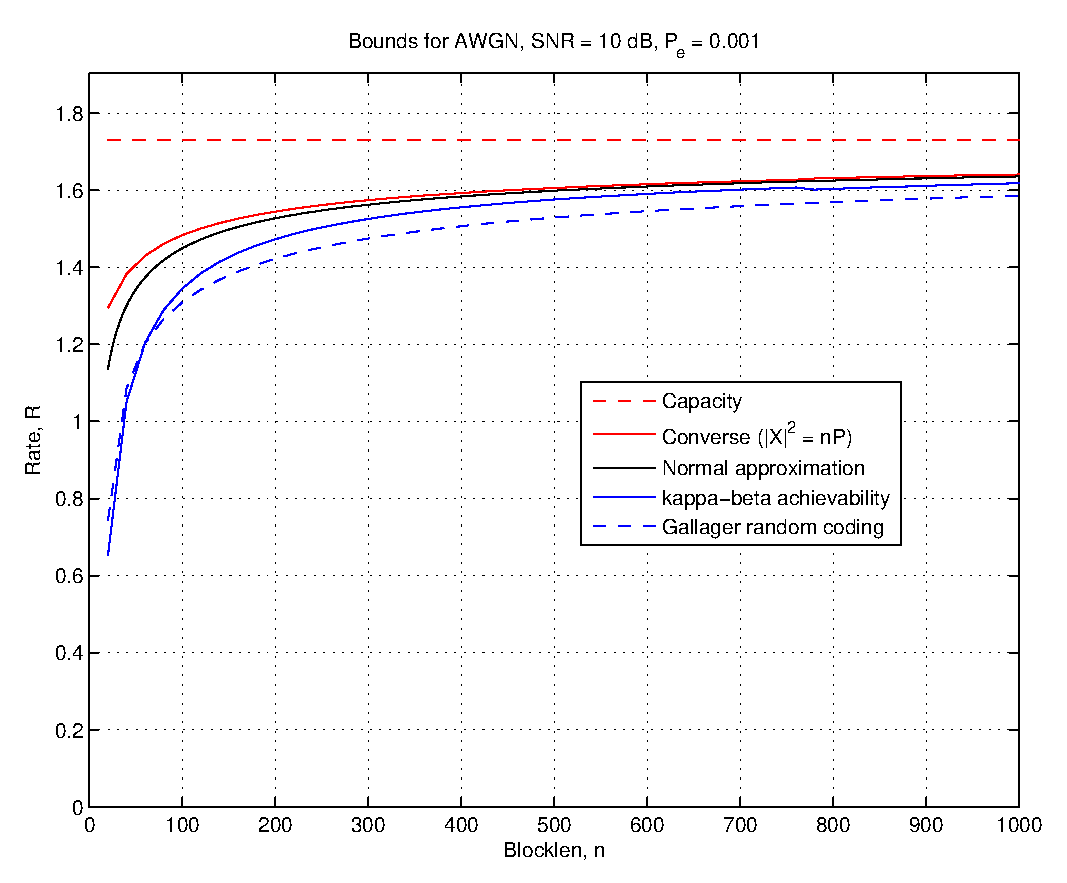
\includegraphics[height=5cm]{plots/awgn_plot3_ex}
\caption{Code and resulting picture for AWGN bounds}\label{fig:awgn_example}
\end{figure}


\section{Summary plot: \texttt{plot\_v3()}}

Definition:
\begin{verbatim}
	function [Ns lb ub feinst gal wlfz] = plot_v3(P, epsil)
\end{verbatim}

This function plots various bounds on the same figure. See Fig.~\ref{fig:awgn_example}.


\section{Achievability: \texttt{shannon\_ach2()}}

Definition:
\begin{verbatim}
	function lm = shannon_ach2(n, epsil, P)
\end{verbatim}

Function computes Shannon's cone-packing achievability bound, see~\cite[(41)]{PPV08}.

\section{Achievability: \texttt{kappabeta\_ach()}}
Format:
\begin{verbatim}
	function Lms = kappabeta_ach(Ns, epsil, P, hack)
\end{verbatim}

This computes the $\kappa\beta$ achievability bound, see left-hand inequality in~\cite[(218)]{PPV08}. If $hack\neq 0$, then we
use asymptotic approximation for $\kappa$. This increases the speed dramatically and is very precise already at $n=10$,
see~\cite[(217)]{PPV08}. If $hack$ is not set, it defaults to $1$.

\section{Achievability: \texttt{gallager\_ach()}}
Format:
\begin{verbatim}
	function lm = gallager_ach(n, epsil, P)
\end{verbatim}

Computes Gallager's achievability bound, see~\cite[(44)]{PPV08}.

\section{Converse: \texttt{converse()}}
Format:
\begin{verbatim}
	function Lms = converse(Ns, epsil, P)
\end{verbatim}

This computes the meta-converse lower bound with $Q_{Y^n} = \matn(0, 1+P)^n$, see right-hand inequality in~\cite[(218)]{PPV08}. 


\section{Normal approximation: \texttt{normapx\_awgn(), normapx\_biawgn()}}

Format:
\begin{verbatim}
	function Lms = normapx_awgn(Ns, epsil, P);
\end{verbatim}

Fast and frequently very precise approximation to both achievability and converse:
	$$ \log M \approx n C - \sqrt{nV} Q^{-1}(\epsilon) + {1\over2} \log n $$


\section{Code database: \texttt{plot\_universe()}}

Code in \verb|universe/plot_universe()| compiles a comparative plot of normalized rate for different codes.
See~\cite[Section IV.D]{PPV08}.



%%%%%%%%%%%%%%%%%%%%%%%%%
\chapter[Block-memoryless Rayleigh fading (no CSI)]{Block-memoryless Rayleigh fading channel, no CSI}

General info:
\begin{itemize}
  \item Maintainer: G. Durisi \url{<durisi@chalmers.se>}
  
  \item Contributors: G. Durisi, J. \"Ostman, W. Yang

  \item Main reference: \cite{durisi14-12a} 

  \item Example: See Fig. \ref{fig:snr6eps03M2}.
  
  \item Channel model: Rayleigh block-fading channel with~$\txant$ 
  transmit antennas and~$\rxant$ receive antennas that stays constant for
   $\cohtime$ channel uses.
  The blocklength $\bl$ is an integer multiple of the coherence time $\cohtime$, i.e., $\bl=\tfdiv\cohtime$; here
  $\tfdiv$ denotes the number of independent time-frequency branches:
  
  \begin{equation}\label{eq:bfmimo}
  	\mathbb{Y}_k = \mathsf{X}_k \mathbb{H}_k + \mathbb{W}_k\,, \qquad k=1,\ldots, \tfdiv\,,
\end{equation}  
  where $\mathbb{Y}_k, \mathbb{W}_k \in \mathbb{C}^{\cohtime \times \rxant}$, $\mathsf{X}_k \in \mathbb{C}^{\cohtime \times
  \txant}$ and $\mathbb{H}_k\in\mathbb{C}^{\txant \times \rxant}$. The noise $\mathbb{W}_k$ and the channel gain
  $\mathbb{H}_k$ are independent and have independent $\mathcal{CN}(0,1)$ entries.
  Neither the transmitter nor the receiver are aware of the realizations of the fading matrix $\mathbb{H}_k$.


  The power constraint is defined \textit{per coherence interval}, i.e., each codeword $\mathsf{C}$  consists of $\tfdiv$ subcodewords $\mathsf{C}_1,\ldots, \mathsf{C}_\tfdiv$ that must
  satisfy:
    \begin{equation*}
      \tr\bigl\{\mathsf{C}_{k}^H \mathsf{C}_{k}\bigr\}= \cohtime\snr,\quad  k=1,\dots,\tfdiv. 
    \end{equation*}
    %
    Here, $\snr$ denotes the SNR. 

  
  \item Common input, output arguments: 
  \begin{itemize}
    \item \verb|snrdB| -- SNR in dB
    \item \verb|T| -- channel coherence time (expressed in channel uses)
    \item \verb|L| -- number of independent fading realizations spanned by each codeword
    \item \verb|Mt| -- number of tranmsmit antennas
    \item \verb|Mr| -- number of receve antennas
    \item \verb|epsilon| -- packet error rate (block error rate)
    \item \verb|prec| -- $\log_2$ of the number of samples used in the Monte-Carlo step; this parameter should be set so that $2^{\verb|prec|} \gg 100 / \verb|epsilon|$
    \item \verb|filename| -- data file in which the samples of the information density are saved for possible future refinements (provided that the flag \verb|SAVE| is set)
    \item \verb|R| -- estimate of the maximum coding rate
    \item \verb|current_eps| -- actual bound on the packet error rate (it may  deviate from \verb|epsilon| if \verb|prec| is not chosen appropriately)
  \end{itemize}
%  [R,current_eps]=DT_USTM_NxM(snrdB,T,L,Mt,Mr,epsilon,prec,filename)
  
\end{itemize}
% section rayleigh_block_fading_channel_with_no_channel_state_information (end)

   \begin{figure}[t]
    \centering
      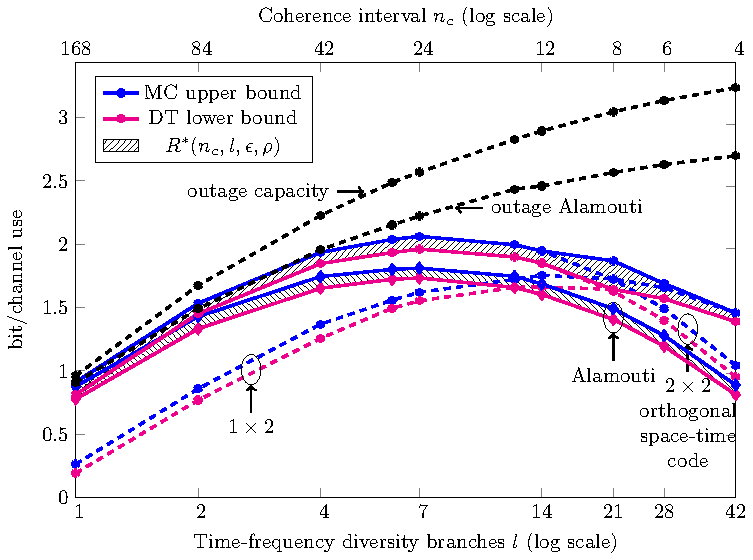
\includegraphics[width=.9\textwidth]{./plots/snr6eps03M2}
    \caption{Maximum coding rate $R^\ast(n_c,l,\epsilon,\rho)$ for $2\times 2$ MIMO system operating over a Rayleigh block-fading channel with coherence time $n_c$.
    Each packet spans~$l$ coherence intervals. The packet size is $168$ channel uses. The packet error rate is $\epsilon=10^{-3}$.
    The SNR is $\rho=6$ dB.}
    \label{fig:snr6eps03M2}
  \end{figure}
  
\section[Achievability bounds]{Achievability bounds: \texttt{DT\_USTM\_NxM()}, \texttt{DT\_USTM\_MxM()}} % (fold)
\label{sec:achievability_bound_dt_ustm_nxm}
%
Format:
\begin{verbatim}
function [R,current_eps]
=DT_USTM(snrdB,T,L,Mt,Mr,epsilon,prec,filename);
\end{verbatim}
%
This  function computes the USTM-DT achievability bound~\cite[Th.~3]{durisi14-12a} for the case $\txant\leq \rxant$.

\section[Converse helper functions]{Converse helper functions: \texttt{MC\_USTM\_2x2\_q1x2()}, \texttt{MC\_USTM\_2x2\_q\_2x2()}, \texttt{MC\_USTM\_4x4\_q\_Mx4}} % (fold)
\label{sec:converse_bounds__texttt}

Format
%
\begin{verbatim}
function [R,current_eps,current_prec]
=MC_USTM_2x2(snrdB,T,L,Mtalt,epsilon,prec,pow_all,filename)
function [R,current_eps,current_prec]
=MC_USTM_4x4(snrdB,Mtalt,T,L,epsilon,prec,pow_all,filename)
\end{verbatim}
%
These two functions compute the right-hand side of~\cite[Eq.~(41)]{durisi14-12a} for fixed input diagonal matrices $\{\Sigma_k\}_{k=1}^{\tfdiv}$ and fixed auxiliary output distribution (which is parameterized by the number of effectively used transmit antennas \verb|Mtalt| that result in this distribution), for the case $\txant=\rxant=2$ and $\txant=\rxant=4$. 
To obtain the actual converse bound, a further optimization over these parameters need to be performed. This is discussed in the next section.
The parameter \verb|pow_all| is related to the diagonal entries of the matrices $\{\Sigma_k\}_{k=1}^{\tfdiv}$. For the $\txant=\rxant=2$ case, \verb|pow_all| is an $\tfdiv$-dimensional vector, whose entries are in $[0,0.5]$. Indeed, the particular formulation of the power constraint in~\cite[Eq.~(41)]{durisi14-12a} implies that the other entry is uniquely determined from the first one.
For the $4\times 4$ case, the code provided assumes that the optimization in~\cite[Eq.~(41)]{durisi14-12a} is restricted only to $\{\Sigma_k\}_{k=1}^{\tfdiv}$ of the form $\Sigma_1=\dots=\Sigma_\tfdiv=\Sigma$. In this case, \verb|pow_all| is a $4$-dimensional vector that contains the diagonal entries of $\Sigma$.
%

\section[Converse bound]{Converse bound: \texttt{compute\_MC\_2x2\_telatar}}
Format
%
\begin{verbatim}
function R=compute_MC_2x2_telatar(snrdB,T,L,epsilon)
\end{verbatim}
%
Compute the metaconverse upper bound~\cite[Eq.~(41)]{durisi14-12a} by invoking the function \texttt{MC\_USTM\_2x2()} and by optimizing over the input diagonal matrices $\{\Sigma_k\}_{k=1}^{\tfdiv}$ and the number of effectively used transmit antennas.
The optimization over the $\{\Sigma_k\}_{k=1}^{\tfdiv}$ is restricted to $2\times 2$ diagonal matrices whose diagonal entries are either [\verb|SNR|$/2$, \verb|SNR|$/2$]  or [\verb|SNR|, 0] according to the generalized form of Telatar conjecture reported in~\cite[Eq.~(42)]{durisi14-12a}.
NOTE: this function may be very slow if \verb|L| is large or \verb|epsilon| is small. 





\section[Alamouti]{Alamouti: \texttt{DT\_USTM\_Alamouti()}, \texttt{MC\_USTM\_Alamouti()}} % (fold)
\label{sec:alamouti}

Format
%
\begin{verbatim}
function [R,current_eps]
=MC_USTM_Alamouti(snrdB,T,L,epsilon,prec,filename)
function [R,current_eps]
=DT_USTM_Alamouti(snrdB,T,L,epsilon,prec,filename)
\end{verbatim}
%
These functions compute achievability and converse bounds for a $2\times 2$ MIMO system with Alamouti used as inner code
%
%
\section[Outage capacity]{Outage: \texttt{outage\_mi()}, \texttt{outage\_alamouti()}, \texttt{outage\_2x2\_telatar()} } % (fold)
\label{sec:outage}
%
\begin{verbatim}
function [Cout,current_eps]
=outage_mi(snrdB,epsilon,Mt,Mr,L,pow_all,prec)  
function [Cout,current_eps]
=outage_alamouti(snrdb,epsilon,L,prec,filename)  
function R=outage_2x2_telatar(L,prec,epsilon,snrdb)
\end{verbatim}
%
The first two functions  compute the outage mutual information $I_{\epsilon}$ for a given set of diagonal input covariance matrices, and the outage mutual
information with Alamouti, respectively:

$$ \PP[ \EE[\imath(X^\tfdiv; \mathbb{Y}^\tfdiv)|\mathbb{H}^\tfdiv] \le
I_\epsilon] = \epsilon\,, $$
where in the first case, the covariance structure of $X^\tfdiv=(X_1,\ldots,X_\tfdiv)$ is specified by \verb|pow_all| and 
$$\imath(X^\tfdiv; \mathbb{Y}^\tfdiv) = \sum_{k=1}^\tfdiv \log {dP_{\mathbb{Y}_k|X_k}\over dP_{\mathbb{Y}_k}}\,.$$
%
The \verb|outage_mi| function evaluates the outage mutual information corresponding to a given input covariance matrix, whose eigenvalues are specified in \verb|pow_all|. Specifically, \verb|pow_all| is a \verb|Mt-1 x L| matrix containing the
first \verb|Mt|$-1$ eigenvalues of the input covariance matrices corresponding to each coherence interval. The last eigenvalue follows from the power constraint. To obtain the outage capacity one has to optimize over all possible choices of $\verb|pow_all|$.

The function \verb|outage_2x2_telatar| provides an example on how to perform this optimization for the $2\times 2$ MIMO case. The optimization is restricted to input covariance matrices that satisfy the generalized Telatar conjecture~\cite[Eq.~(42)]{durisi14-12a} according to which in 
the eigenvalues of the input covariance matrix in each coherence interval satisfy the following property: $k$ out the \verb|Mt| eigenvalues are equal to \verb|SNR|$/k$ and the remaining \verb|Mt|$-k$ eigenvalues are equal to zero. The value of $k$ may change across the coherence intervals.


\section[Ergodic capacity]{Ergodic capacity: \texttt{ergodic\_USTM()}}
\begin{verbatim}
function RergUSTM=ergodic_USTM(snrdB,T,Mt,Mr,prec)
\end{verbatim}
This function computes a lower bound on the ergodic capacity (no CSIR), obtained by evaluating the mutual information for a USTM input distribution. 
It is assumed that $\txant\leq\rxant$.


%%%%%%%%%%%%%%%%%%%%%%%%%%%%%%
\chapter{Quasi-static fading channel}

\label{ch:qs-fading-st}



General info:
\begin{itemize}
\item Maintainer: W. Yang \url{<weiy@princeton.edu>}

\item Main references: \cite{yang14-07a}

\item Example: See Fig.~\ref{fig:bounds-simo}

\item Channel model: a quasi-static MIMO fading channel with $\txant$ transmit and $\rxant$ receive antennas. The channel input-output relation within $\bl$ channel uses is given by 
\begin{equation}
\mathbb{Y} = \mathsf{X}\mathbb{H} + \mathbb{Z}
\end{equation}
where $\mathsf{X} \in\complexset^{\bl\times\txant}$ is the signal transmitted over $\bl$ channel uses; $\mathbb{Y} \in \complexset^{\bl\times\rxant}$ is the corresponding received signal; the matrix $\mathbb{H}\in\complexset^{\txant\times\rxant}$ contains the complex fading coefficients, which are random but remain constant over the~$\bl$ channel uses;
%
 $\mathbb{Z} \in \complexset^{\bl\times\rxant}$ denotes the additive noise at the receiver, which is independent of $\mathbb{H}$ and has iid $\mathcal{CN} (0,1)$ entries. 
	Power constraints: each codeword $x^n$ satisfies
			$$ \|\mathsf{X} \|_{\mathrm{F}}^2 \le n P .$$
In the code, we also assume that  the entries of $\mathbb{H}$ are iid Rician-distributed, i.e., 
$$H_{ij} \sim \mathcal{CN} (\sqrt{K/(K+1)}, 1/(K+1))$$
where $K$ is the Rician $K$-factor. 

\item The code for the MIMO case ($\txant>1$) is built under the additional assumption that all codewords $\mathsf{X}$ are ``isotropic'', i.e.,  (see~\cite[Sec.~III]{yang14-07a})
\begin{equation}
\label{eq:mimo-iso-constraint}
 \frac{1}{\bl} \mathsf{X}^{\mathrm{H}} \mathsf{X} = \frac{P}{\txant} \mathsf{I}_{\txant}.
 \end{equation}
Currently, we do not have code for MIMO achievability and converse bounds that hold without the assumption~\eqref{eq:mimo-iso-constraint}.


\item Input/output arguments:
\begin{enumerate}
\item \verb|nn| -- input argument; vector of blocklengths.
\item \verb|error| -- input argument; block error probability.
\item \verb|tx|, \verb|rx| -- input arguments; number of transmit and receive antennas.
%\item \verb|rx| -- input argument; number of receive antennas.
\item \verb|P| -- input argument; parameter of the power constraint (linear scale).
\item \verb|K| -- input argument; Rician $K$-factor. If \verb|K| is not set, it defaults to $0$, in which case the entries of $\mathbb{H}$ follow a Rayleigh distribution.
\item \verb|rate_a|, \verb|rate_c|, \verb|rate_na| -- output arguments; lower (achievability) bound, upper (converse) bound, and normal approximation of  $(\log_2 M)/n$, channel coding rate (base-2 information units).
%\item \verb -- output argument; upper (converse) bound on $(\log_2 M)/n$.
%\item \verb|rate_na| -- output argument; normal approximation of $(\log_2 M)/n$. 
\end{enumerate}

\end{itemize}


\begin{figure}[t]
	\centering
	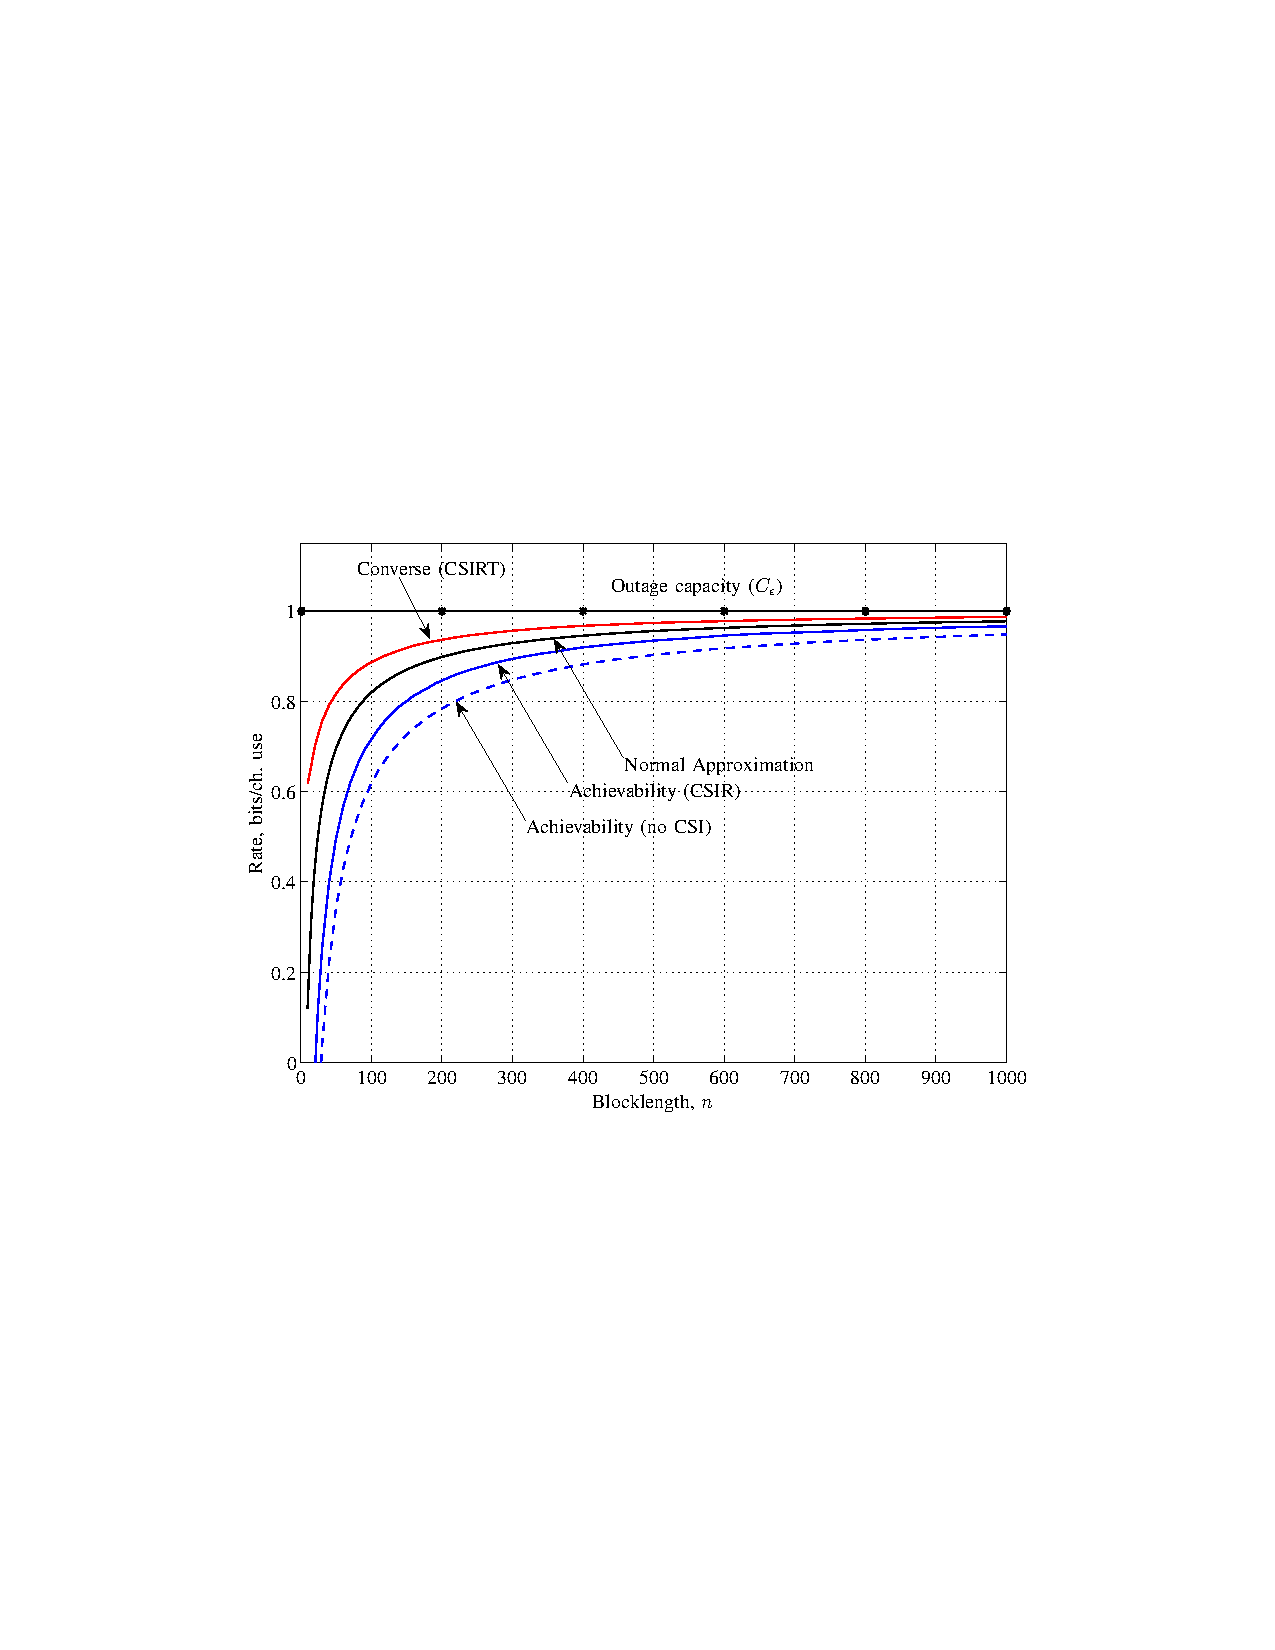
\includegraphics[scale=0.5]{plots/quasi-static-simo.pdf}
\vspace{-1.5mm}
\caption{Achievability and converse bounds for a quasi-static SIMO Rician-fading channel with $K$-factor equal to $20$ dB, two receive antennas, $\text{SNR}=-1.55 $ dB, and $\epsilon=10^{-3}$. 
\label{fig:bounds-simo}}
\end{figure}


%\section{Summary plot: \texttt{plot\_v3()}}
%
%Definition:
%\begin{verbatim}
%	function [Ns lb ub feinst gal wlfz] = plot_v3(P, epsil)
%\end{verbatim}
%
%This function plots various bounds on the same figure. See Fig.~\ref{fig:awgn_example}.
\section{Summary plot: \texttt{plot\_all()}}

Format:
\begin{verbatim}
[C_e, rate_a, rate_c, rate_na] = plot_all(nn, P, error, tx, rx, K);
\end{verbatim}

This function plots capacity/achievability/converse/normal approximation curves on the same figure. See Fig.~\ref{fig:bounds-simo}.


\section{Achievability: \texttt{ach\_simo\_csir()}}

Format:
\begin{verbatim}
	function rate_a = ach_simo_csir(nn, P, error, rx, K);
\end{verbatim}

This function computes the $\kappa\beta$ achievability bound over a single-input multiple-output (SIMO) channel with perfect CSIR, see~\cite[Footnote~7]{yang14-07a}.

\section{Achievability: \texttt{ach\_simo\_nocsi()} }
Format:
\begin{verbatim}
	function rate_a = ach_simo_nocsi(nn, P, error, rx, K);
\end{verbatim}

This function computes the achievability bound over a SIMO channel with no CSI, see~\cite[Eq.~(67)]{yang14-07a}. 

\section{Achievability: \texttt{mimo\_iso\_ach()}}
Format:
\begin{verbatim}
	function rate_a = mimo_iso_ach(nn, P, error, tx, rx, K);
\end{verbatim}

This function computes the achievability bound over a MIMO channel with no CSI, where all input codewords satisfy $\mathsf{X}^{\mathrm{H}}\mathsf{X} = \frac{\bl P}{\txant}\mathsf{I}_{\txant}$, see~\cite[Eq.~(65)]{yang14-07a}. 

\section{Converse: \texttt{converse\_simo()}}
\begin{verbatim}
	function rate_c = converse_simo(nn,P, error, rx, K);
\end{verbatim}

This function computes the converse bound over a single-input multiple-output (SIMO) channel with CSIRT, see~\cite[Eq.~(76)]{yang14-07a}.

\section{Converse: \texttt{mimo\_iso\_conv()}}
\begin{verbatim}
	function rate_c = mimo_iso_ach(nn, P, error, tx, rx, K);
\end{verbatim}

This function computes the converse bound over a MIMO channel with CSIRT, where all input codewords satisfy $\mathsf{X}^{\mathrm{H}}\mathsf{X} = \frac{\bl P}{\txant}\mathsf{I}_{\txant}$, see~\cite[Eq.~(78)]{yang14-07a}. 



\section[Normal approximation]{Normal approximation: \texttt{normapprox\_simo()}, \texttt{normapprox\_mimo\_iso()}}

Format:
\begin{verbatim}
	function rate_na = normapprox_simo(nn,P, error, rx, K)
	function rate_na = normapprox_mimo_iso(nn, P, error, tx, rx, K);
\end{verbatim}

These two functions compute the normal approximation $R^{\mathcal{N}}(\epsilon,\bl)$ to both achievability and converse, obtained by solving the following equation
	$$ \epsilon  =\mathbb{E}\mathopen{}\left[Q\mathopen{}\left(\frac{C(\mathbb{H}) - R^{\mathcal{N}}(\epsilon,\bl) }{\sqrt{ n V(\mathbb{H}) }}\right)\right]$$
where
$$C(\mathsf{H}) \triangleq \log_2 \mathrm{det}\mathopen{} \left(\mathsf{I}_{\txant} + \frac{P}{\txant} \mathsf{H} \mathsf{H}^{H} \right)$$
and
$$V(\mathsf{H}) \triangleq  m\log_2^2 e  - \sum\limits_{i=1}^{m } \frac{\log_2^2 e}{(1+P\lambda_i/\txant)}$$
with $m \triangleq \min\{\txant , \rxant\}$ and $\{\lambda_i\}$ being the eigenvalues of $\mathsf{H}\mathsf{H}^{\mathrm{H}}$.



\chapter{Quasi-static fading channel (long-term power constraint) }

General info:
\begin{itemize}
\item Maintainer: W. Yang \url{<weiy@princeton.edu>}

\item Main references: \cite{yang15-09}

%\item Example: See Fig.~\ref{fig:ebno_example} 

\item Channel model:
\begin{equation}
Y_i = H X_i + Z_i, \qquad i=1,\ldots, n
\label{eq:qs-channel-lt}
\end{equation}
where 
\begin{itemize}
%
\item $X_i, Y_i \in \complexset$ are the channel input and output, respectively
%
\item $H\in \complexset$ is the complex channel coefficient 
%
\item $ Z_i \sim \mathcal{CN}(0,1)$ is the i.i.d. white Gaussian noise
\end{itemize}
%
%
\item An $(n,M,\epsilon)_{\mathrm{lt}}$ code for the channel~\eqref{eq:qs-channel-lt} consists of 
%
\begin{itemize}
\item an encoder $f:\{1,\ldots,M\} \times \complexset \to \complexset^n $ that maps the message $W\in\{1,\ldots,M\}$ and the channel coefficient $H$ to a codeword $x^n = f(W,H)$ satisfying the \emph{long-term}  (i.e., averaged-over-all-codeword) power constraint 
\begin{equation}
\mathbb{E}_{W,H}\mathopen{}\big[\|f(W,H)\|^2\big] \leq n P
\end{equation}
where $W$ is equiprobable on $\{1,\ldots,M\}$ 
%
\item a decoder $g: \complexset^n \times \complexset \to\{1,\ldots,M\}$ satisfying the average error probability constraint 
\begin{equation}
\mathbb{P}[g(Y^n , H) \neq W] \leq \epsilon
\end{equation}
where $Y^n$ is the channel output induced by the transmitted codeword $x^n = f(W,H)$ according to~\eqref{eq:qs-channel-lt}.
 \end{itemize}

\item Remark: for comparison, a code is said to satisfy a \emph{short-term}  (i.e., per-codeword) power constraint if the encoder satisfies 
\begin{equation}
\|f(W,H)\|^2 \leq n P 
\end{equation}
with probability one, see Chapter~\ref{ch:qs-fading-st}. 

\item Common input/output arguments:
\begin{itemize}
\item \verb|snr_db| -- input argument; SNR in dB
\item \verb|nn| -- input argument; blocklength
\item \verb|error| -- input argument; block error probability
\item \verb|rate_ach_lt|/\verb|rate_conv_lt|/\verb|rate_na_lt| -- output arguments; lower (achievability) bound, upper (converse) bound, and normal approximation of $(\log_2 M)/n$, maximal achievable rate (in bits/ch. use).

\end{itemize}



\end{itemize}



\section{The AWGN channel ($H=1$)}

Format 

\begin{verbatim}
	function rate_ach_lt=awgn_ach_lt(snr_db, nn, error);
	function rate_conv_lt=awgn_conv_lt(snr_db, nn, error);
	function rate_na_lt = awgn_na_lt(snr_db,nn,error);
\end{verbatim}

These functions compute achievability/converse/normal approximation of $(\log_2 M)/n$, maximal achievable rate (in bits/ch. use). The bounds are from~\cite[Section II.C]{yang15-09} .

\section{Quasi-static fading channel with perfect CSIT}

Under construction.  


\chapter{Block-memoryless Rayleigh Fading (CSIR)}

General info:
\begin{itemize}
\item Maintainer: A. Collins \url{<austinc@mit.edu>}

\item Main references: Coming Soon

\item Example: See Figure~\ref{fig:block_mimo_summary}

\item Channel Model: with $n_t$ transmit antennas, $n_r$ receive antennas, and coherence time $T$, the model is given by
\begin{align*}
Y_j = H_jX_j + Z_j, \qquad j = 1,\hdots,n
\end{align*}
Where $\mathbb{F}$ is either $\mathbb{R}$ or $\mathbb{C}$, and
\begin{itemize}
\item $X_j \in \mathbb{F}^{n_t \times T}$ is channel input
\item $H_j \in \mathbb{F}^{n_r \times n_t}$ is fading matrix, iid Rayleigh per block
\item $Z_j \in \mathbb{F}^{n_r \times T}$ is the i.i.d. (circularly symmetric) Gassian noise matrix.
\item $Y_j \in \mathbb{F}^{n_r \times T}$ is output matrix
\end{itemize}
The input must satisfy the per-codeword power constraint
\begin{align*}
\sum_{j=1}^n \|x_j\|_F^2 \leq nP
\end{align*}

\item Input / output arguments
\begin{itemize}
\item \verb|P| -- Power constraint
\item \verb|n| -- number of coherent blocks (for $nT$ total channel uses)
\item \verb|n_t| -- number of transmitter antennas
\item \verb|n_r| -- number of receiver antennas
\item \verb|T| -- channel coherence time (in number of channel uses)
\item \verb|epsilon| -- average probability of error
\item \verb|real_or_complex| -- specifies real or complex channel (set to \verb|'real'| or \verb|'complex'|, respectively)
\end{itemize}
\end{itemize}

\section{Summary plot: \texttt{plot\_all()}}

Format:
\begin{verbatim}
    function log_M = plot_all(P,n_t,n_r,T,epsilon)
\end{verbatim}

This will plot the achievability bound, the normal approximation, and the capacity as in Figure~\ref{fig:block_mimo_summary}.  To change the plot range, the \verb|n_vec| vector can be changed to include the desired points.

\begin{figure}[ht]\label{fig:block_mimo_summary}
    \centering
    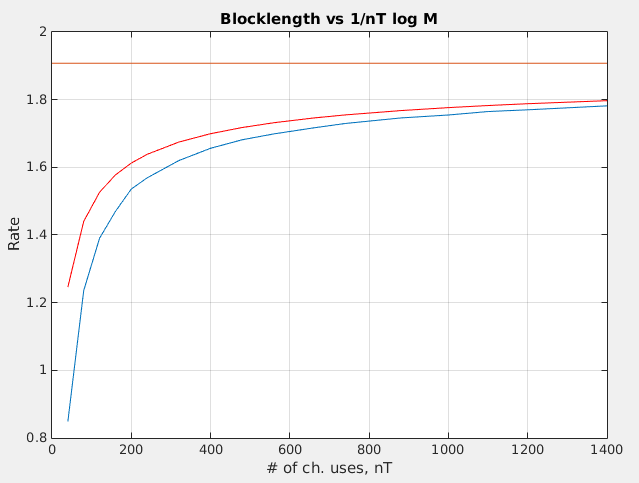
\includegraphics[scale=0.50]{plots/block-csir-mimo.png}
\vspace{-1.5mm}
\caption{Achievability (blue), normal approximation (red), and capacity for the real MIMO CSIR block fading channel with $n_t = n_r = T = 2$, $P=10$, $\epsilon = 10^{-3}$.
\label{fig:bounds-simo}}
\end{figure}


\section{Achievability Bound: \texttt{MIMO\_achievability\_CSIR()}}

Format:
\begin{verbatim}
    function log_M = MIMO_achievability_CSIR(n,epsilon,n_t,n_r,T,P,real_or_complex)
\end{verbatim}

This function computes the following average probability of error achievability bound:

\begin{align*}
\log M \geq \sup_{0<\tau<\epsilon} \sup_{Q_Y}\frac{\beta_{\tau}(P_Y,Q_Y)}{\beta_{1-\epsilon+\tau}(P_{XY},P_XQ_Y)}
\end{align*}
Where $P_Y$ is the output distribution through the channel when the input $P_X$ has the following distribution ($X^n$ iid $\mathcal{N}(0,P/n_t)$)
\begin{align*}
X^n \frac{\sqrt{nTP}}{\|X^n\|_F}
\end{align*}
And $Q_Y$ is the output distribution when the input is iid Gaussian $\mathcal{N}(0,P/n_t)$.  Both of these are fairly easily adjustable in the code.

Note that the \verb|iter| variable in the code sets the number of Monte Carlo iterations.  The sampling loop uses \verb|parfor|, which attempts to distribute the computation.  The number of Monte Carlo iterations should be taken $~< 100/\epsilon$.  For small $\epsilon$ (e.g. $10^{-3}$, you may want to let the code run overnight.

\section{Normal Approximation: \texttt{MIMO\_csir\_normapx()}}

Format:
\begin{verbatim}
    function logM = MIMO_csir_normapx(n,epsilon,n_t,n_r,T,P,real_or_complex)
\end{verbatim}

This function computes the normal approximation up to the $O(\sqrt{n})$ term, i.e.
\begin{align*}
\log M \approx nTC - \sqrt{nTV}Q^{-1}(\epsilon)
\end{align*}
It utilizes one of two functions to compute the capacity $C$ and dispersion $V$:
\begin{verbatim}
    function [C,V] = capacity_and_dispersion(n_t,n_r,T,P)
\end{verbatim}
or
\begin{verbatim}
    function [C,V] = capacity_and_dispersion_mc(n_t,n_r,T,P,real_or_complex)
\end{verbatim}
The \verb|capacity_and_dispersion| function computes $C$ and $V$ via numerical integration for the complex MIMO channel, while \verb|capacity_and_dispersion_mc| compute these quantities using Monte Carlo.  The Monte Carlo computation is also useful it's flexibility, e.g. it's simple to change the fading distribution to compute the capacity and dispersion of non-Rayleigh fading channels.



\chapter{Energy-per-bit under vanishing spectral efficiency}

General info:
\begin{itemize}
\item Maintainer: Y. Polyanskiy \url{<yp@mit.edu>}

\item Main references: \cite{PPV10eneff,YDP15}

\item Example: See Fig.~\ref{fig:ebno_example} 

\item Channel model:
\begin{equation}\label{eq:ebno_channel}
		Y_j = H_j X_j + Z_j, \quad j=1,\ldots \qquad n=\infty \quad\mbox{\bfseries (!!!)} 
\end{equation}	
	\begin{itemize}
	\item Noise: $Z_j \sim \matcn(0,N_0)$ iid and $N_0$ is noise spectral density
	\item Channel gain (for AWGN): $H_j=1$ constant
	\item Channel gain (for Rayleigh fading): $H_j\sim\matcn(0,1)$ iid 
	\item Power constraints: Each codeword $x^\infty$ satisfies
			$$ \sum_{j=1}^\infty |x_j|^2 \le E\,,  $$
		where $E$ is the total energy budget. 
	\item Energy-per-bit: For the codebook $\matc$ of size $M$ its energy-per-bit is defined as
			$$ E_b = {E\over \log_2 M}\,.$$
	\end{itemize}

\item Description: \\Bounds in this Chapter address the question of finding the absolutely minimal energy-per-bit required
for transmitting $\log_2 M$ bits with probability of error $\epsilon$ and \textit{without
restriction on the number of channel uses}. Asymptotically as $M\to \infty$ it is known:
	$$ {E_b\over N_0} \to \log_e 2 \approx -1.59~dB $$

\item Real/Complex: In the regime of infinite bandwidth as here, there is no difference between real/complex channel
inputs (but noise variance in the real case should be taken $Z_j \sim \matn(0, {N_0\over 2})$).

\item MIMO and block-fading: Surprisingly, having multiple transmit antennas or block-constant fading makes no 
	difference for energy-per-bit, see~\cite{YDP15}. Having $m_r>1$ receive antennas is equivalent to scaling $N_0
	\to {N_0\over m_r}$ and thus again does not require any special treatment.

\item Remark: These bounds correspond to allowing no feedback link. Even a modicum of feedback significantly
improves the energy-per-bit tradeoff at finite length, see~\cite{PPV10eneff}.

\item Remark: The tradeoff $E_b\over N_0$ vs. $\log_2 M$ can also be interpreted as the rate-blocklength tradeoff for the
power-constrained \textit{infinite-bandwidth} continunuous-time channel, see~\cite[(50)-(51)]{PPV10eneff}.

\item Common input/output arguments:
\begin{enumerate}
\item \verb|epsil| -- block probability of block error.
\item \verb|lm| or \verb|Lms| -- input or output argument; $\log_2 M$, log-size of codebook (base-2 information units). 
\item \verb|en0| or \verb|EE| -- input/output argument; total energy budget available \verb|EE|$={E\over N_0}$ (to get ${E_b\over
N_0}$ divide by \verb|lm|).
\end{enumerate}
\end{itemize}

\section{Summary plot}

\begin{verbatim}
	plot_all()
\end{verbatim}

This script generates two figures, shown on Fig.~\ref{fig:ebno_example}.

\textbf{Note:} Script takes several hours to finish.

\begin{figure}
\centering
\begin{verbatim}
	> energy-per-bit/plot_all()
\end{verbatim}

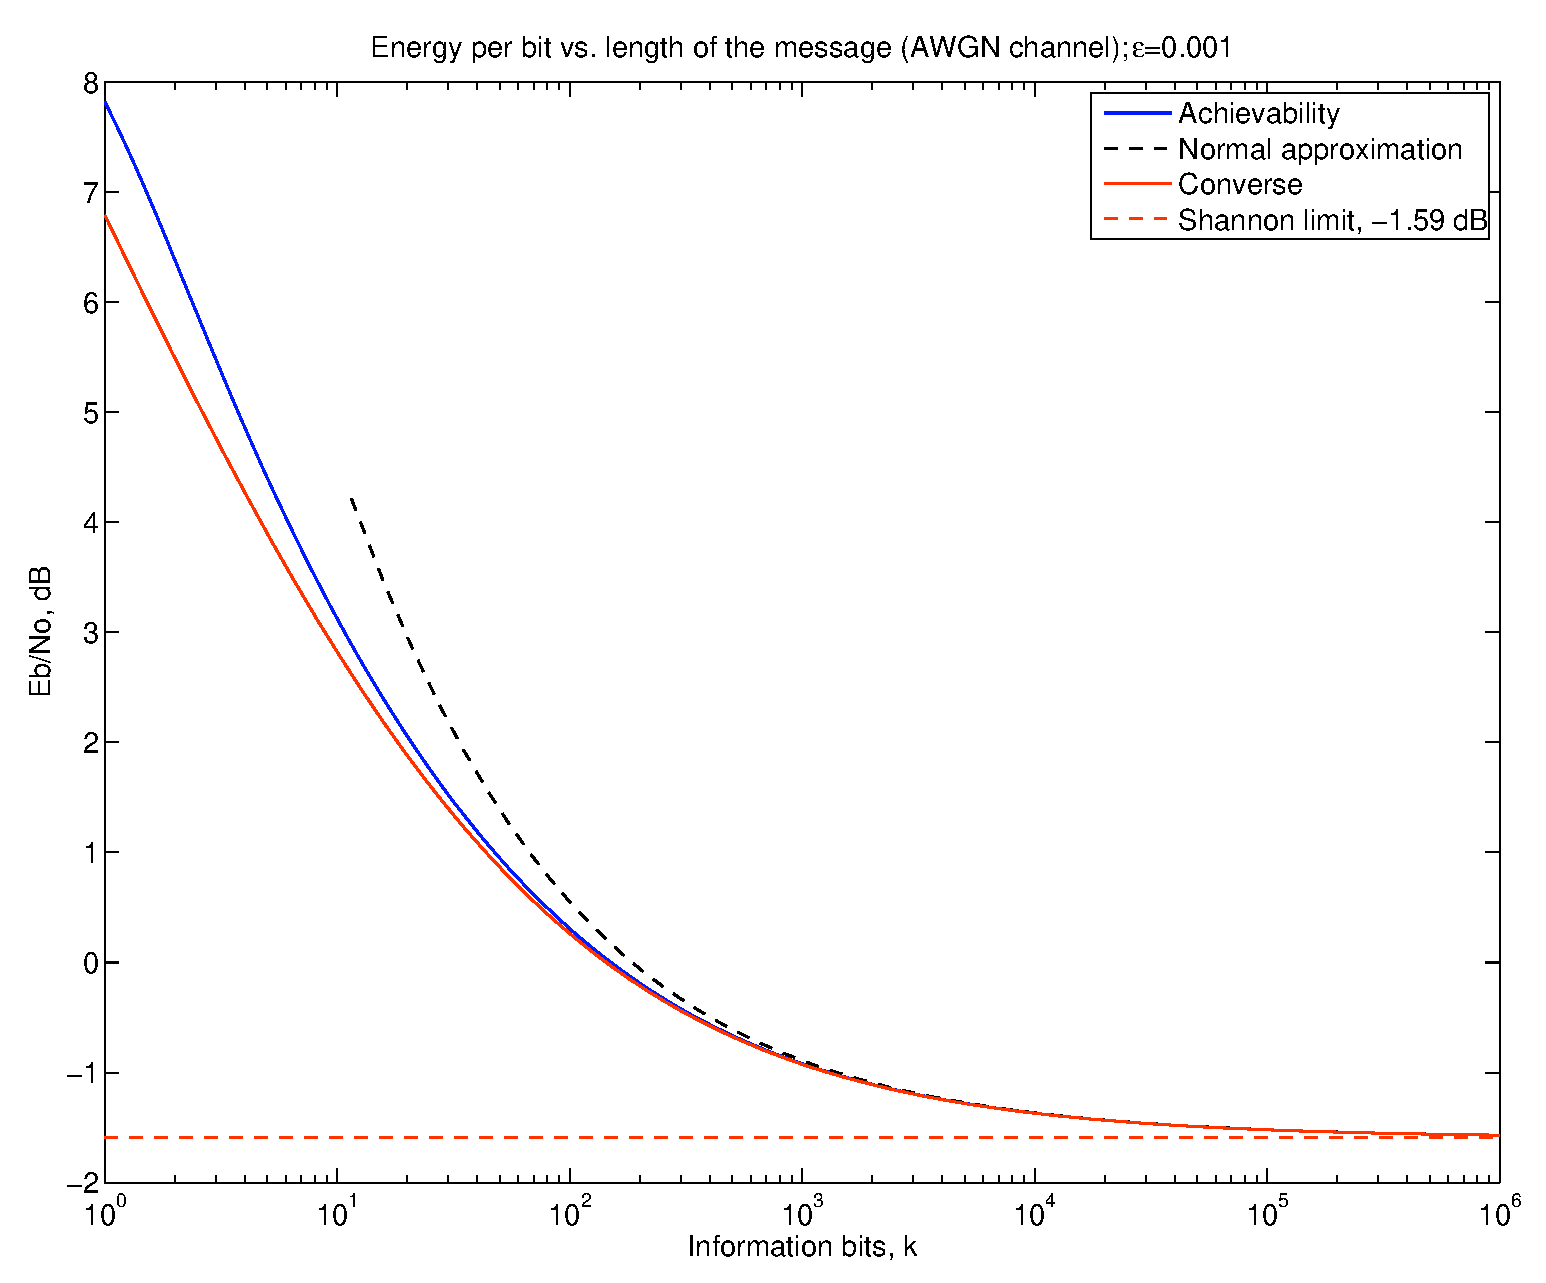
\includegraphics[width=.4\textwidth]{plots/energy_awgn}
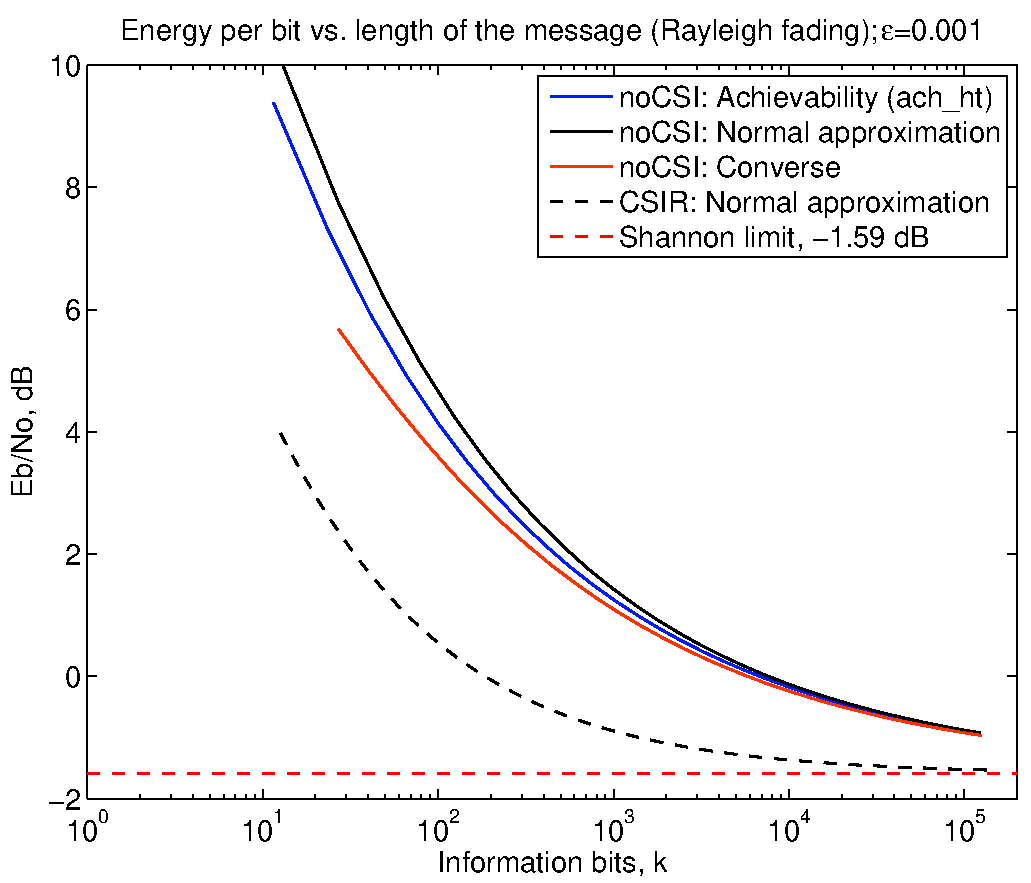
\includegraphics[width=.4\textwidth]{plots/energy_nocsi}
\caption{Example figures generated by the energy-per-bit code}\label{fig:ebno_example}
\end{figure}

\section{The AWGN channel ($H_j=1$)}

Here $H_j=1$ in the channel model~\eqref{eq:ebno_channel}.

Format:
\begin{verbatim}
	function En0 = energy_awgn_ach(Lms, epsil);
	function lm = energy_awgn_conv(en0, epsil);
	function lm = energy_awgn_normapx(en0, epsil);
\end{verbatim}

These functions return achievability/converse/normal approximation. The bounds are from~\cite[Theorems 2 and 3]{PPV10eneff}.

\section{Rayleigh fading: CSIR case}

Format:
\begin{verbatim}
	function lm = energy_csir_conv(EE, epsil);
\end{verbatim}

This function computes the converse (upper) bound on the number of information bits, \verb|lm|, that a Rayleigh fading
channel with perfect CSIR can transmit under a total energy budget \verb|EE|$={E\over N_0}$; see~\cite[Theorem
11]{YDP15}. Note that for CSIR case we can use \verb|energy_aegn_ach()| and \verb|energy_awgn_normapx()| for
achievability and normal approximation, see~\cite[Section III.D]{YDP15}.

\medskip
\textbf{Note:} vector \verb|EE| should be in ascending order.

\section{Rayleigh fading: noCSI case}

Format:
\begin{verbatim}
	function lm = energy_nocsi_ach_ht(EE, epsil);
	function lm = energy_nocsi_ach_ml(EE, epsil);
\end{verbatim}

	These are two achievability bounds~\cite[Corollary 4 and 5]{YDP15} with the second one, \verb|_ml()|, being
	typically better.

\begin{verbatim}
	function lm = energy_nocsi_conv(EE, epsil);
	function lm = energy_nocsi_normapx(EE, epsil);
\end{verbatim}

	The converse bound is~\cite[Theorem 6]{YDP15}. The normal approximation is computed by maximizing over $A$
	in~\cite[(64)]{YDP15}.

\medskip
\noindent\textbf{Note:} Vector \verb|EE| should be in ascending order.\\
\textbf{Note:} Functions \verb|energy_nocsi_ach_ml()| and \verb|energy_nocsi_conv()| are \textit{very slow}. 



% subsection outage_outage_capacity()_outage_capacity_alamouti()_ (end)








\chapter{Fixed-length source coding under a distortion criterion}

\begin{itemize}
\item Maintainer: V. Kostina \url{<vkostina@caltech.edu>}

\item Main references: \cite{kostina2011fixed}

\item Performance criterion - excess distortion probability: $$ \PP[ \mathsf d(S, Z) > d] \leq \epsilon,$$
where $S$ is the source and $Z$ is its representation. 


\item The code uses auxiliary functions contained in \verb|lib/|. This directory can to be added to Matlab path by running the following command: \verb|path(path, '../../lib');|

\item To speed up calculations, some functions use the so-called `persistent' variables whose values are retained during multiple calls to those functions. This helps to choose the starting positions for various optimizations wisely. For example, if the function is computed for blocklength $510$ after blocklength $500$, it takes advantage of the previous computation to choose a starting position for various optimizations. To avoid problems, use command \verb|clear all| to clear the values of all persistent variables when making a computation unrelated to the previous computation.    


\item Recommended usage: 
\begin{verbatim}
path(path, '../../lib');
clear all; 

N = 10:10:1000;
out = NaN(1, length(N));
for k = 1:length(N)
    n = N(k);  
    try
        out(k) = Rstar(..., n, ...);  
        save('mydatafile');  
    catch ME
        fprintf('Error: %s\n', getReport(ME));
        out(k) = NaN;
    end    
end
\end{verbatim}


\item For an example plot (produced via~\verb|sc/GMS/plot_all.m|) see Fig.~\ref{fig:cgms1}.
\begin{figure}
\centering
\begin{verbatim}
	> cd sc/GMS
	> plot_all(0.1, 0.01, 10:5:500)
\end{verbatim}
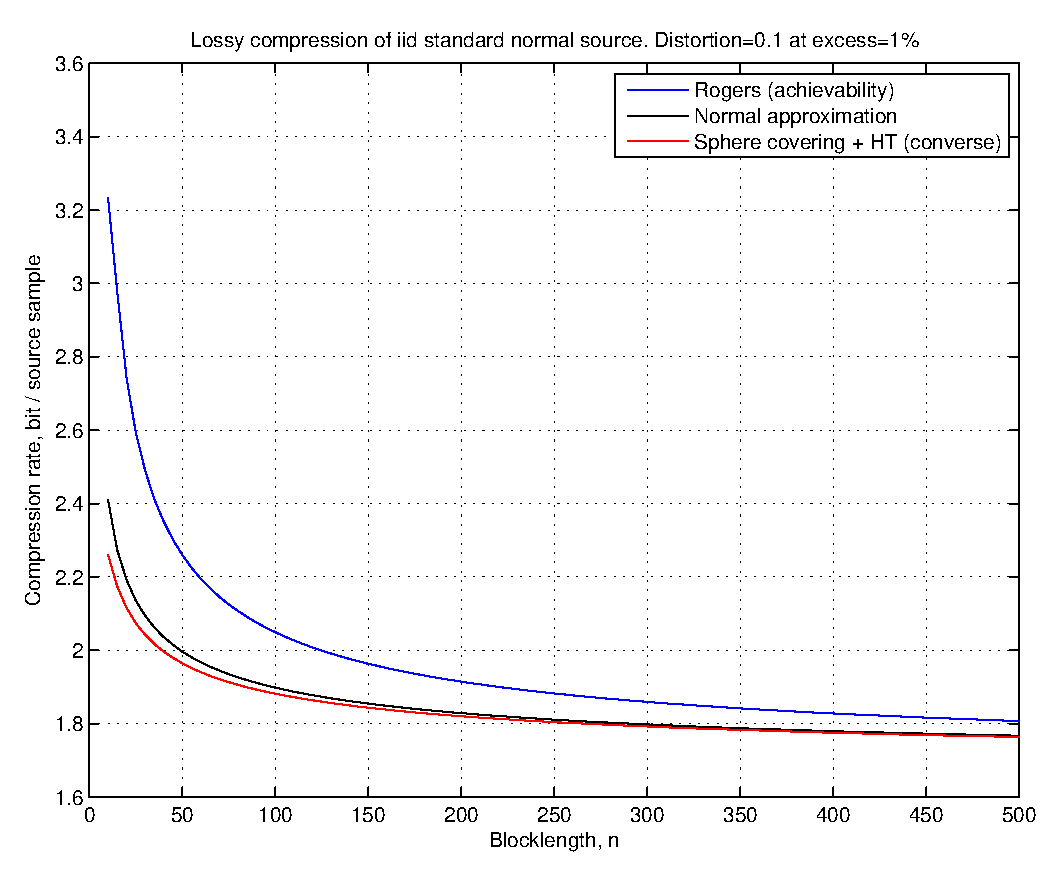
\includegraphics[height=5cm]{plots/compress_gms}
\caption{Lossy compression bounds for the memoryless Gaussian source.}\label{fig:cgms1}
\end{figure}

\end{itemize}





\section{Binary memoryless source}

\subsection{Source model}
$ S_1, S_2, \ldots $ are i.i.d Bernoulli with bias $p$. 

\subsection{Distortion measure}
Bit error rate $$\mathsf d(s^k, z^k) = \frac 1 k \sum_{i = 1}^k 1\{s_i \neq z_i\}.$$

\subsection{Matlab code}
 \verb|sc/BMS/|


\subsection{Main functions}
\begin{description}
\item[\texttt{Rstar(d, n, e, p, fun)}:]  Compression rate compatible with a given excess distortion. 
\item[\texttt{Dstar(R, n, e, p, fun)}:]  Distortion threshold compatible with a given excess probability and a given rate. 
\end{description}

\subsection{Input arguments}

\begin{description}
\item[\texttt{d}:] distortion threshold.
\item[\texttt{R}:] compression rate.
\item[\texttt{n}:] blocklength.
\item[\texttt{e}:] excess distortion probability.
\item[\texttt{p}:] source bias.
\item[\texttt{fun}:] alias for the function to be computed. Acceptable values:
\begin{description}
\item \emph {`shannon'}: Shannon's achievability bound \cite[Theorem 1]{kostina2011fixed}.
\item \emph {`normal'}: Gaussian approximation \cite[Theorem 12]{kostina2011fixed}.
\item \emph {`spherecoveringc'}: Converse via sphere covering and hypothesis testing \cite[Theorem 8]{kostina2011fixed}.
\item \emph {`generalc'}: General converse via $\mathsf d$-tilted information \cite[Theorem 7]{kostina2011fixed}.
\item \emph {`spherecoveringa'}: Achievability via covering with random spheres  \cite[Theorem 21]{kostina2011fixed}.
\item \emph {`permutationa'}: Achievability via permutation coding (i.e. all codewords are of the same type, namely, the type that achieves the rate-distortion function)  \cite[Theorem 22]{kostina2011fixed}.
\item \emph {`martona'}: Converse via Marton's bound \cite[Theorem 5]{kostina2011fixed}.
\end{description}
\end{description}








\section{Gaussian memoryless source}

\subsection{Source model}
$ S_1, S_2, \ldots $ are i.i.d $\mathcal N(0, 1)$. 

\subsection{Distortion measure}
Squared error $$\mathsf d(s^k, z^k) = \frac 1 k \sum_{i = 1}^k (s_i - z_i)^2$$

\subsection{Matlab code}
\verb|sc/GMS/|


\subsection{Main functions}
\begin{description}
\item[\texttt{Rstar(d, n, e, fun)}:]  Compression rate compatible with a given excess distortion. 
\item[\texttt{Dstar(R, n, e, fun)}:]  Distortion threshold compatible with a given excess probability and a given rate. 
\end{description}

\subsection{Input arguments}

\begin{description}
\item[\texttt{d}:] distortion threshold.
\item[\texttt{R}:] compression rate.
\item[\texttt{n}:] blocklength.
\item[\texttt{e}:] excess distortion probability.
\item[\texttt{fun}:] alias for the function to be computed. Acceptable values:
\begin{description}
\item \emph {`shannon'}: Shannon's achievability bound \cite[Theorem 1]{kostina2011fixed}.
\item \emph {`normal'}: Gaussian approximation \cite[Theorem 12]{kostina2011fixed}.
\item \emph {`spherecoveringc'}: Converse via sphere covering and hypothesis testing \cite[Theorem 8]{kostina2011fixed}.
\item \emph {`spherecoveringa'}: Achievability via covering with random spheres \cite[Theorem 37]{kostina2011fixed}.
\end{description}

The following \texttt{fun} values are accepted only by \texttt{Rstar(...)}.
\begin{description}
\item \emph {`generalc'}: General converse via $\mathsf d$-tilted information \cite[Theorem 7]{kostina2011fixed}. 
\item \emph {`rogersa'}: Achievability using a result by Rogers \cite[Theorem 39]{kostina2011fixed}.
\end{description}


\end{description}





\section{Binary erased source}

\subsection{Source model}
$ S_1, S_2, \ldots $ are i.i.d fair coin flips. However, the encoder does not observe $S_1, S_2, \ldots$. Instead, it observes an erased version of the source: $X_1, X_2, \ldots$, where $X_i = S_i$ with probability $1 - \alpha$, and $X_i = \texttt{?}$ with probability $\alpha$.    

\subsection{Distortion measure}
Bit error rate with respect to the original source$$\mathsf d(s^k, z^k) = \frac 1 k \sum_{i = 1}^k 1\{s_i \neq z_i\}, \qquad s_i, z_i \in \{ \texttt{0, 1} \}. $$

\subsection{Matlab code}
 \verb|sc/BES/|


\subsection{Main functions}
\begin{description}
\item[\texttt{Rstar(d, n, e, alpha, fun)}:]  Compression rate compatible with a given excess distortion. 
\end{description}

\subsection{Input arguments}

\begin{description}
\item[\texttt{d}:] distortion threshold.
\item[\texttt{n}:] blocklength.
\item[\texttt{e}:] excess distortion probability.
\item[\texttt{alpha}:] erasure probability. 

\item[\texttt{fun}:] alias for the function to be computed. Acceptable values:
\begin{description}
\item \emph {`spherecoveringa'}: Achievability via covering with random spheres  \cite[Theorem 33]{kostina2011fixed}.
\item \emph {`spherecoveringc'}: Converse via sphere covering (hypothesis testing) \cite[Theorem 32]{kostina2011fixed}.
\item \emph {`normal'}: Gaussian approximation \cite[Theorem 12]{kostina2011fixed}.
\item \emph {`aeq'}: Achievability via covering with random spheres for a surrogate rate-distortion problem which negates the stochastic variability of the erasure channel \cite{kostina2013ITWnoisysc}.
\item \emph {`ceq'}: Converse via sphere covering (hypothesis testing) for the surrogate problem \cite{kostina2013ITWnoisysc}. 
\item \emph {`normaleq'}: Gaussian approximation for the surrogate problem \cite{kostina2013ITWnoisysc}.
\end{description}
\end{description}









\chapter{Variable-length compression allowing errors}

\begin{itemize}
\item Maintainer: V. Kostina \url{<vkostina@caltech.edu>}

\item Main references: \cite{kostina2015varrate}.


\item Fixed probability of error: $$ \PP[ S \neq Z ] \leq \epsilon,$$
where $S$ is the source and $Z$ is its reconstruction after the (almost lossless) encoding.

\item Performance criterion: average length of the compressed representation.   

\item Performance criterion - excess distortion probability: $$ \PP[ \mathsf d(S, Z) > d] \leq \epsilon,$$
where $S$ is the source and $Z$ is its reconstruction after the transmission over a noisy channel. 
\item The code uses auxiliary functions contained in \verb|lib/|. This directory needs to be added to Matlab path by running the following command: \verb|path(path, '../../lib');|

\item To speed up calculations, some functions use the so-called `persistent' variables whose values are retained during multiple calls to those functions. This helps to choose the starting positions for various optimizations wisely. For example, if the function is computed for blocklength $510$ after blocklength $500$, it takes advantage of the previous computation to choose a starting position for various optimizations. To avoid problems, use command \verb|clear all| to clear the values of all persistent variables when making a computation unrelated to the previous computation.    


\item Recommended usage: 
\begin{verbatim}
path(path, '../../lib');
clear all; 

N = 10:10:1000;
out = NaN(1, length(N));
for k = 1:length(N)
    n = N(k);  
    try
        out(k) = Rstar(..., n, ...);  
        save('mydatafile');  
    catch ME
        fprintf('Error: %s\n', getReport(ME));
        out(k) = NaN;
    end    
end
\end{verbatim}


\end{itemize}




\section{Binary memoryless source}
\subsection{Source model}
$ S_1, S_2, \ldots $ are i.i.d Bernoulli with bias $p$. 


\subsection{Matlab code}
 \verb|sc/varrate/|
 
 
 
 
 \subsection{Main function}
\begin{description}
\item[\texttt{Rstar(p, e, n, fun)}:]  Compression rate compatible with a given excess distortion. 
\end{description}

\subsection{Input arguments}

\begin{description}
\item[\texttt{p}:] source bias.
\item[\texttt{e}:] error probability.
\item[\texttt{n}:] blocklength.
\item[\texttt{fun}:] alias for the function to be computed. Acceptable values:
\begin{description}
\item \emph {`approx'}:  Gaussian approximation \cite[Theorem 4]{kostina2015varrate}.
\item \emph {`exact'}: Exact minimum average rate \cite[(26)]{kostina2015varrate}.
\item \emph {`exacti'}: Exact value of the Erokhin function  \cite[(40)]{kostina2015varrate}.
\item \emph {`ie'}: Exact value of the expectation of the $\epsilon$-cutoff of information in $S^k$  \cite[(11),(13)]{kostina2015varrate}.
\end{description}

\end{description}

 
 
 
 
 
 
 
 
 
 
\chapter{Joint source-channel coding under a distortion criterion}

\begin{itemize}
\item Maintainer: V. Kostina \url{<vkostina@caltech.edu>}

\item Main references: \cite{kostina2012jscc}

\item Performance criterion - excess distortion probability: $$ \PP[ \mathsf d(S, Z) > d] \leq \epsilon,$$
where $S$ is the source and $Z$ is its reconstruction after the transmission over a noisy channel. 
\item The code uses auxiliary functions contained in \verb|lib/|. This directory needs to be added to Matlab path by running the following command: \verb|path(path, '../../lib');|

\item To speed up calculations, some functions use the so-called `persistent' variables whose values are retained during multiple calls to those functions. This helps to choose the starting positions for various optimizations wisely. For example, if the function is computed for blocklength $510$ after blocklength $500$, it takes advantage of the previous computation to choose a starting position for various optimizations. To avoid problems, use command \verb|clear all| to clear the values of all persistent variables when making a computation unrelated to the previous computation.    


\item Recommended usage: 
\begin{verbatim}
path(path, '../../lib');
clear all; 

N = 10:10:1000;
out = NaN(1, length(N));
for k = 1:length(N)
    n = N(k);  
    try
        out(k) = Rstar(..., n, ...);  
        save('mydatafile');  
    catch ME
        fprintf('Error: %s\n', getReport(ME));
        out(k) = NaN;
    end    
end
\end{verbatim}


\end{itemize}





\section{Binary memoryless source transmitted over a binary symmetric channel}

\subsection{Source model}
$ S_1, S_2, \ldots $ are i.i.d Bernoulli with bias $p$. 


\subsection{Channel model}
$Y_i = X_i + N_i$, where $N_i$ are i.i.d. Bernoulli with bias $\delta$. 


\subsection{Distortion measure}
Bit error rate $$\mathsf d(s^k, z^k) = \frac 1 k \sum_{i = 1}^k 1\{s_i \neq z_i\}.$$

\subsection{Matlab code}
 \verb|jscc/BMS-BSC/|


\subsection{Main functions}
\begin{description}
\item[\texttt{Rstar(p, delta, d, e, n, fun)}:]  Compression rate compatible with a given excess distortion. 
\item[\texttt{Dstar(R, n, e, p, delta, fun)}:]  Distortion threshold compatible with a given excess probability and a given rate. 
\end{description}

\subsection{Input arguments}

\begin{description}
\item[\texttt{p}:] source bias.
\item[\texttt{delta}:] channel crossover probability.
\item[\texttt{d}:] distortion threshold.
\item[\texttt{e}:] excess distortion probability.
\item[\texttt{R}:] compression rate.
\item[\texttt{n}:] blocklength.
\item[\texttt{fun}:] alias for the function to be computed. Acceptable values:
\begin{description}
\item \emph {`approx'}:  Gaussian approximation \cite[Theorem 10]{kostina2012jscc}.
\item \emph {`clistdecoding'}: Converse via list decoding and hypothesis testing \cite[Theorem 4]{kostina2012jscc}.
\item \emph {`ajoint'}: Achievability via joint source-channel coding  \cite[Theorem 8]{kostina2012jscc}.
\item \emph {`aseparate'}: Achievability via separation  \cite[Theorem 6]{kostina2012jscc}.
\end{description}


The following \texttt{fun} values are accepted only by \texttt{Rstar(...)}.
\begin{description}
\item \emph {`cgeneral'}: General converse via $\mathsf d$-tilted information \cite[Theorem 2]{kostina2012jscc}.
\item \emph {`approxseparate'}: Gaussian approximation for the separation architecture  \cite[(126)]{kostina2012jscc}.
\item \emph {`arcu'}: For the almost lossless transmission, achievability via RCU bound  \cite[Theorem 9]{kostina2012jscc}.
\end{description}
The following \texttt{fun} values are accepted only by  \texttt{Dstar(...)}. 
\begin{description}
\item \emph {`random'}: Achievability via random coding for fair coin flip source \cite[Theorem 6]{kostina2012jscc}.
\item \emph {`nocoding'}: Achievability via no coding.  \cite[Theorem 23]{kostina2012jscc}.
\end{description}


\end{description}






\section{Gaussian source transmitted over an AWGN channel}

\subsection{Source model}
$ S_1, S_2, \ldots $ are i.i.d $\mathcal N(0, 1)$. 


\subsection{Channel model}
$Y_i = X_i + N_i$, where $N_i$ are i.i.d. $\mathcal N(0, 1)$. 


\subsection{Distortion measure}
Squared error $$\mathsf d(s^k, z^k) = \frac 1 k \sum_{i = 1}^k (s_i - z_i)^2.$$

\subsection{Matlab code}
 \verb|jscc/GMS-AWGN/|


\subsection{Main functions}
\begin{description}
\item[\texttt{Rstar(P, d, e, n, fun)}:]  Transmission rate compatible with a given excess distortion (nats). 
\item[\texttt{Dstar(R, n, e, P, fun)}:]  Distortion threshold compatible with a given excess probability and a given rate. 
\end{description}

\subsection{Input arguments}

\begin{description}
\item[\texttt{P}:] maximum allowable transmit power, or SNR.
\item[\texttt{d}:] distortion threshold.
\item[\texttt{e}:] excess distortion probability.
\item[\texttt{R}:] transmission rate.
\item[\texttt{n}:] blocklength.
\item[\texttt{fun}:] alias for the function to be computed. Acceptable values:


\begin{description}
\item \emph {`approx'}:  Gaussian approximation \cite[Theorem 10]{kostina2012jscc}.
\item \emph {`cht'}: Converse via list decoding and hypothesis testing \cite[Theorem 4]{kostina2012jscc}.
\item \emph {`ajoint'}: Achievability via joint source-channel coding  \cite[Theorem 8]{kostina2012jscc}.
\item \emph {`aseparate'}: Achievability via separation  \cite[Theorem 6]{kostina2012jscc}.
\end{description}


The following \texttt{fun} values are accepted only by \texttt{Dstar()}. 
\begin{description}
\item \emph {`nocoding'}: Achievability via no coding \cite[Theorem 24]{kostina2012jscc}.
\item \emph {`approxnocoding'}: Gaussian approximation for the uncoded system \cite[(129), (208)]{kostina2012jscc}.
\end{description}

The following \texttt{fun} values are accepted only by \texttt{Rstar()}.
\begin{description}
\item \emph {`cgeneral'}: General converse via $\mathsf d$-tilted information \cite[Theorem 2]{kostina2012jscc}.
\item \emph {`approxseparate'}: Gaussian approximation for the separation architecture  \cite[(126)]{kostina2012jscc}.
\end{description}

\end{description}






%%%%%%%%%%%%%%%%%%%%%%%%%%%%
\bibliographystyle{IEEEtran}
\bibliography{IEEEabrv,refs}
\end{document}

